%%%%%%%%%%%%%%%%%%%%%  kbb talk %%%%%%%%%%%%%%%%%%%%%%%%%%%%%%%
%%%%%%%%%%%%%%%%%%%%%%%%%%%%%%%%%%%%%%%%%%%%%%%%%%%%%%%%%%%%%%%

\documentclass[12pt,fleqn]{seminar}
\input{seminar.bug}
\pagestyle{empty}
\pdfhorigin=1truein
\pdfvorigin=1truein


% packages
\usepackage{ifpdf}
\usepackage{bm}
\usepackage{latexsym}
\usepackage{color}
\usepackage{pstricks}
\usepackage{ulem} %uwave
\usepackage{amsmath}

\usepackage{amssymb}
%\usepackage{float}
\usepackage{bm}
%\usepackage{wasysym}
%\usepackage[landscape]{geometry}
\usepackage{graphicx}
\usepackage{epstopdf}
\graphicspath{{./Figs/}{./}{../}}

\begin{document}


% basic	commands I
\newcommand{\mass}{\mathsf{M}} 
\newcommand{\half}{\mbox{\small $\frac{1}{2}$}}
\newcommand{\sinc}{\mbox{sinc}}
\newcommand{\const}{\mbox{const}}
\newcommand{\trc}{\mbox{trace}}
\newcommand{\intt}{\int\!\!\!\!\int }
\newcommand{\ointt}{\int\!\!\!\!\int\!\!\!\!\!\circ\ }
\newcommand{\eexp}{\mbox{e}^}
\newcommand{\bra}{\left\langle}
\newcommand{\ket}{\right\rangle}
\newcommand{\EPS} {\mbox{\LARGE $\epsilon$}}
\newcommand{\ttimes} {\mbox{\tiny \ $^{\times}$ \ }}
\newcommand{\ar}{\mathsf r}
\newcommand{\im}{\mbox{Im}}
\newcommand{\re}{\mbox{Re}}
\newcommand{\bmsf}[1]{\bm{\mathsf{#1}}} 
\newcommand{\pd}[2]{\frac{\partial #1}{\partial #2}}
\newcommand{\bitem}{$\newline \ \ \bullet \ \ $} 
\newcommand{\ola}{\protect\overleftarrow}
\newcommand{\ora}{\protect\overrightarrow}

% basic	commands II
\newcommand{\hide}[1]{}
\newcommand{\tbox}[1]{\mbox{\tiny #1}}
\newcommand{\Cn}[1]{\begin{center}{#1}\end{center}}
\newcommand{\be}{\begin{eqnarray*}}
\newcommand{\ee}{\end{eqnarray*}}
\newcommand{\beq}{\begin{eqnarray*}}
\newcommand{\eeq}{\end{eqnarray*}}

\newcommand{\mpg}[2][0.45\hsize]{\begin{minipage}[b]{#1}{#2}\end{minipage}}
%
\newcommand{\bmp}[1]{\begin{minipage}[t]{#1}\noindent }
\newcommand{\smp}[1]{\end{minipage}\begin{minipage}[t]{#1}\noindent }
\newcommand{\emp}{\end{minipage}}

\newcommand{\amatrix}[1]{\begin{matrix} #1 \end{matrix}} 


% extra commands for colors
\definecolor{blk}{rgb}{0.,0.,0.}
\definecolor{red}{rgb}{1.,0.,0.}
\definecolor{green}{rgb}{0.,0.5,0.}
\definecolor{blue}{rgb}{0.,0.,1.}
\definecolor{bluek}{rgb}{0.,0.,0.5}
\definecolor{orange}{rgb}{1.,0.56.,0}
\newcommand{\cblk}[1]{\textcolor{blk}{#1}}
\newcommand{\cred}[1]{\textcolor{red}{#1}}
\newcommand{\cgreen}[1]{\textcolor{green}{#1}}
\newcommand{\cblue}[1]{\textcolor{blue}{#1}}
\newcommand{\cbluek}[1]{\textcolor{bluek}{#1}}
\newcommand{\corange}[1]{\textcolor{orange}{#1}}


% extra commands for slides

%\newcommand{\Up}[1][0.5]{\vspace{-#1cm}}
%\newcommand{\Dn}[1][0.5]{\vspace{#1cm}}
%\newcommand{\Tl}[1]{\begin{center}{\bf \small \cblue{#1}}\end{center}}

\newcommand{\Up}[1][5]{\vspace{-#1mm}}
\newcommand{\Dn}[1][5]{\vspace{#1mm}}
\newcommand{\Tl}[1]{\begin{center}{\bf \small \cblue{#1}}\end{center}}

\renewcommand{\slideparindent}{0mm}
\setlength{\mathindent}{0cm} 

% \newcommand{\newsld}{\end{slide}\begin{slide}}


\newcommand{\bslA}[1]{
%portrait
\pdfpagewidth=210truemm
\pdfpageheight=297truemm
\pdfhorigin=1truein
\pdfvorigin=1truein
%portrait
\renewcommand{\slidetopmargin}{0mm}
\renewcommand{\slideleftmargin}{-54mm}
\setlength{\slidewidth}{190mm}
\setlength{\slideheight}{277mm}
\begin{slide}
}



\newcommand{\bslB}[1]{
%landscape
\pdfpagewidth=297truemm
\pdfpageheight=210truemm
\pdfhorigin=1truein
\pdfvorigin=1truein
%portrait 
\renewcommand{\slidetopmargin}{0mm}
\renewcommand{\slideleftmargin}{33mm}
\setlength{\slideheight}{190mm}
\setlength{\slidewidth}{150mm} %130
%portrait fonts
\begin{slide}
\ptsize{8}
}



\newcommand{\bslC}[1]{
%landscape
\pdfpagewidth=297truemm
\pdfpageheight=210truemm
\pdfhorigin=1truein
\pdfvorigin=1truein
%landscape
\renewcommand{\slidetopmargin}{0mm}
\renewcommand{\slideleftmargin}{33mm}
\setlength{\slideheight}{190mm}
\setlength{\slidewidth}{277mm}
%portrait fonts
\begin{slide}
\ptsize{8}
}



\newcommand{\bslD}[1]{
%landscape
\pdfpagewidth=297truemm
\pdfpageheight=210truemm
\pdfhorigin=1truein
\pdfvorigin=1truein
%landscape
\renewcommand{\slidetopmargin}{0mm}
\renewcommand{\slideleftmargin}{33mm}
\setlength{\slideheight}{190mm}
\setlength{\slidewidth}{277mm}
%landscape fonts
\begin{slide}
}



\newcommand{\esl}{\end{slide}}


\newcommand{\vbar}{
\begin{picture}(1,1)
\thicklines
\put(0,61){ \ \ \line(0,-1){280} \ \ } 
\end{picture} 
}


%%%%%%%%%%%%%%%%%%%%%%%%%%%%%%%%%%%%%%%%%%%%%%%%%%%%%%%%%%%%%%%%%%%
%%%%%%%%%%%%%%%%%%%%%%%%%%%%%%%%%%%%%%%%%%%%%%%%%%%%%%%%%%%%%%%%%%%


%%%%%%%%%%%%%%%%%%%%%%%%%%%%%%%%%%%%%%%%%%%%%%%%%%%%%%%%%%%%%%%%%%%
%%%%%%%%%%%%%%%%%%%%%%%%%%%%%%%%%%%%%%%%%%%%%%%%%%%%%%%%%%%%%%%%%%%

%%%%%%%%%%%%%%%%%%%%%%%%%%%%%%%%
\bslD

\Tl{\Large{Percolation, sliding, localization and relaxation in glassy circuits }}


\Cn{\bf Daniel Hurowitz, Doron Cohen,\\ \corange{Ben-Gurion University}}
%
%
%\bmp{0.5\hsize}
%
%
%
%%\Cn{ \includegraphics[ height=4cm]{}}
%
%\smp{0.5\hsize}
%
%\vspace{0.2cm}
%
%
%
%%{\includegraphics[height=3cm]{ResistorsNetworkBath_a}}
%
%\emp
%
%\bmp{\hsize}



\bmp{0.5\hsize}

\Cn{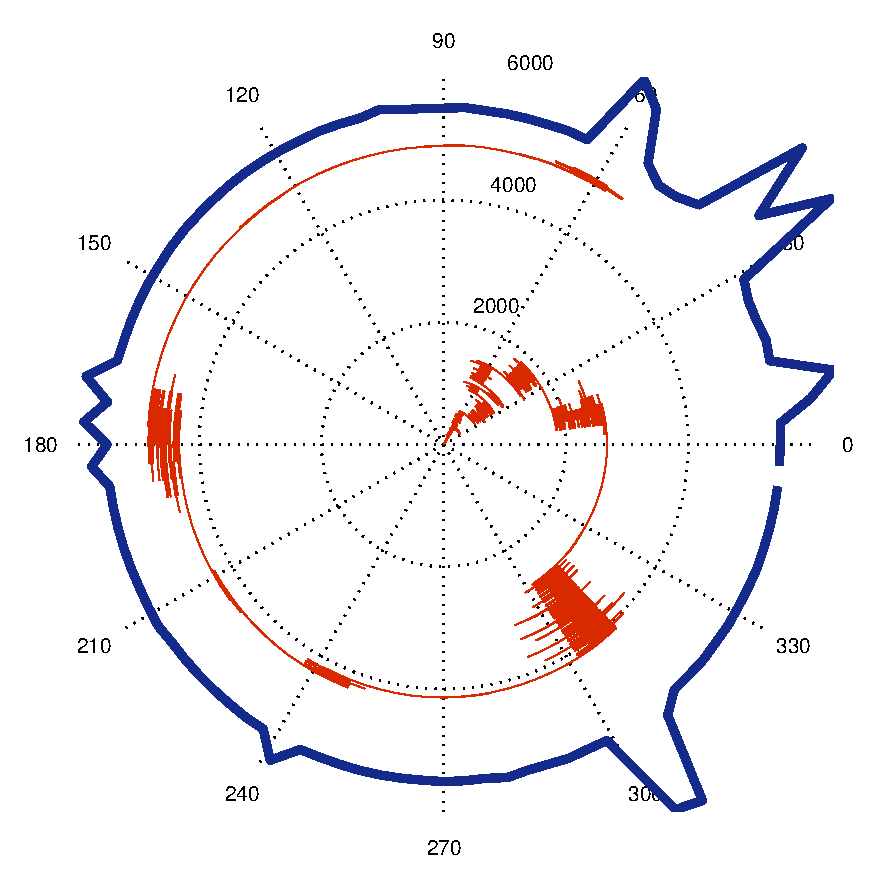
\includegraphics[height=5cm]{/Figs/polar_1_a.eps}}

\smp{0.5\hsize}

\Cn{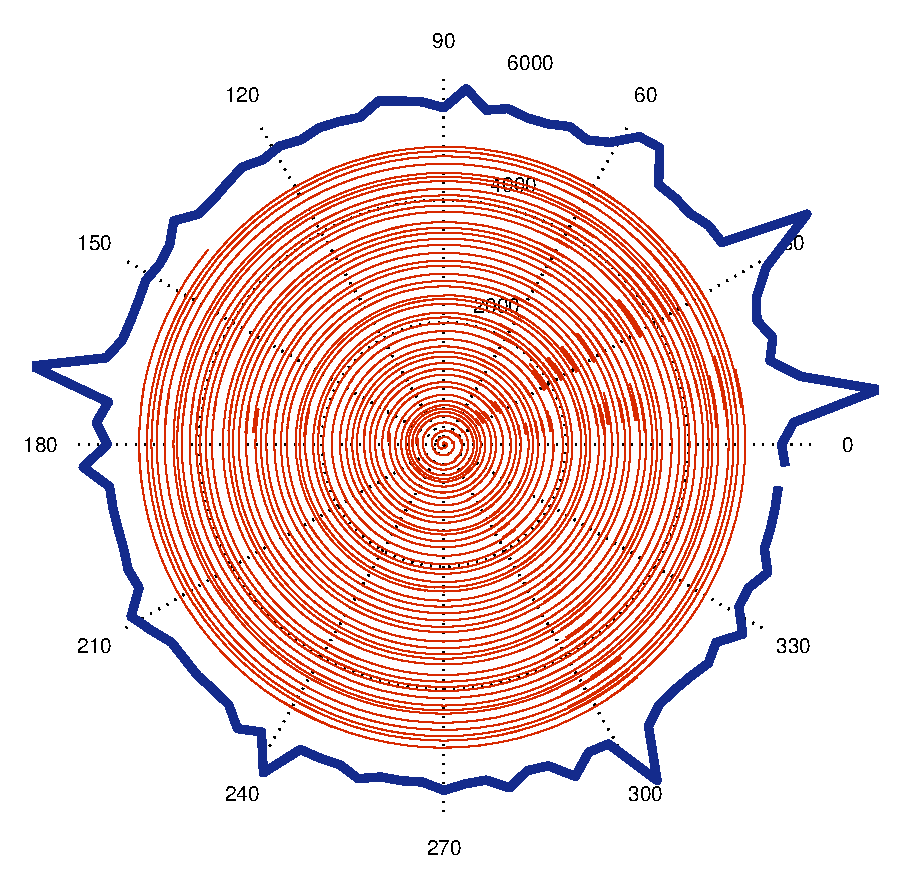
\includegraphics[height=5cm]{/Figs/polar_2_a.eps}}

\emp



%\emp

\esl


%%%%%%%%%%%%%%%%%%%%%%%%%%%%%%%%
\bslC

\Tl{\large Brownian motion}

\Dn[2]

\cgreen{The Einstein-Smoluchowski Relation (ESR):}

\Up

\beq
\hspace{5cm} D = \mu k_B T, \ \ \ \ \ \ \ \ \ \ k_B=1
\eeq

Relation between mobility ($\mu$) and diffusion ($D$) reflecting microscopics ($k_B$) in universal way.

This is a special case of a \cred{fluctuation-dissipation relation} between first and second moments.



\beq
\text{\cgreen{Drift:}} \ \  && \langle x \rangle \ = \ vt, \ \ \ \ \ \ \  v \ = \ \mu F  \\
\text{\cgreen{Diffusion:}} \ \  && \text{Var}(x) \ = \ 2Dt \\
\text{\cgreen{ESR:}} \ \ && \frac{v}{D} \ \ = \ \  \frac{F}{T} \ \ \equiv \ \ s \ \ = \ \ \mbox{\cgreen{affinity (linear response)}}
%\ \ \ \ \ \cgreen{\leadsto} \ \ \ \ \  \frac{\mu}{D} \ = \ \frac{1}{T}
\eeq

\Dn

$s \ \equiv \ $ \cgreen{entropy-production-per-distance}  

\Dn

\center{\cred{\bf FDT is valid close to equilibrium.}}

\center{\cred{\bf To what extent does the ESR hold? }}

\center{\cred{\bf Can it be derived from the NFT? }}

\center{\cred{\bf Non-equilibrium version?}}

\esl



%%%%%%%%%%%%%%%%%%%%%%%%%%%%%%%%%%%%%%%%%%%%%%%%%

\bslC

\Tl{\large{Sinai spreading}}

\bmp{0.55\hsize}

\Up

\be
\cgreen{\text{Stochastic field:}} \ \ 
\mathcal{E}_n \ \equiv \ \ln \left[\frac{\ora{w}_n}{\ola{w_n}}\right]  \ ,  
\hspace{1cm} \cred{\sigma = \sqrt{\mbox{Var} (\mathcal{E}_n)}}
\ee


\be
\text{\cgreen{Stochastic Motive Force:} } \ \ 
\mathcal{S}_{\circlearrowleft} = 
\sum_{n\in\text{ring}} \ \ln \left[ \ \frac{\ora{w}_n}{\ola{w}_n} \ \right ] 
\ee

\be
\text{\cgreen{If}} \ \ \ \frac{\ora{w}_n}{\ola{w}_n}=\exp\left[-\frac{E_n-E_{n-1}}{T} \right] 
\ \ \ \cgreen{\leadsto} \ \ \  
\mathcal{S}_{\circlearrowleft}  \ = \ 0
\ee


\be
\text{\cgreen{Affinity}}: \ \ s \  = \ \frac{\mathcal{S}_{\circlearrowleft}}{N}
\ee


\Dn


\cgreen{For small $s$} [1]:

Sub-diffusive spreading $x \ \sim \ [\log (t)]^2$,

Exponentially small drift $\displaystyle v  \ \sim \ e^{-\sqrt{N}}$.
 

\Dn

\cgreen{For arbitrary $s$} [2,3]: 

Complicated expressions for $v$ and $D$.

\Dn

\cgreen{For a periodic lattice, no disorder:}

\Up

\[
 \frac{v}{D} \  \ =  \ \ \frac{2}{a} \tanh\left(\frac{as}{2}\right)
\]


\smp{0.45\hsize}

\hspace*{1cm}
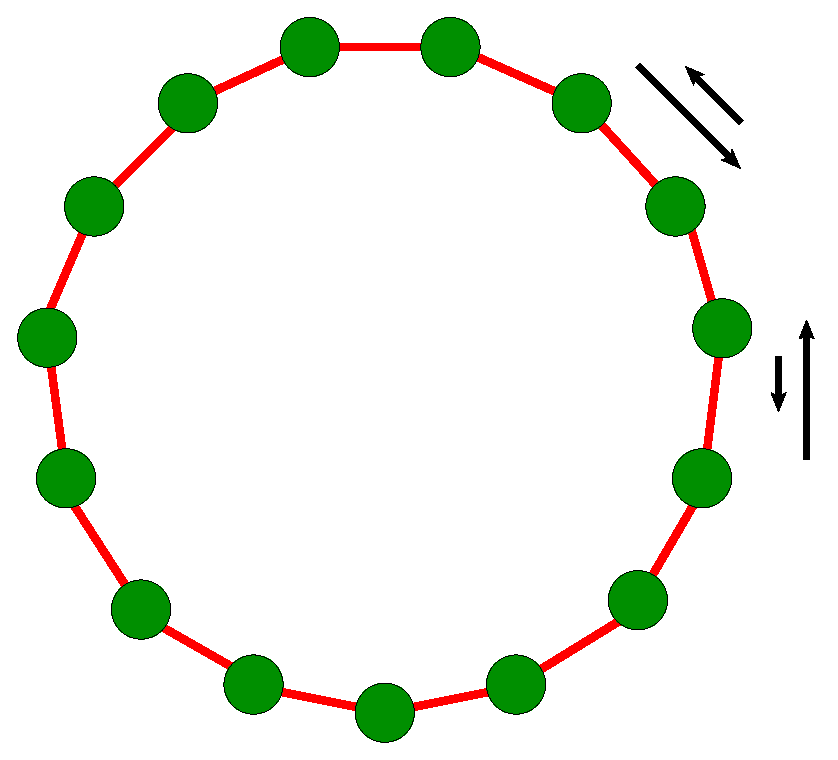
\includegraphics[height=25mm]{sparse_network2.eps}

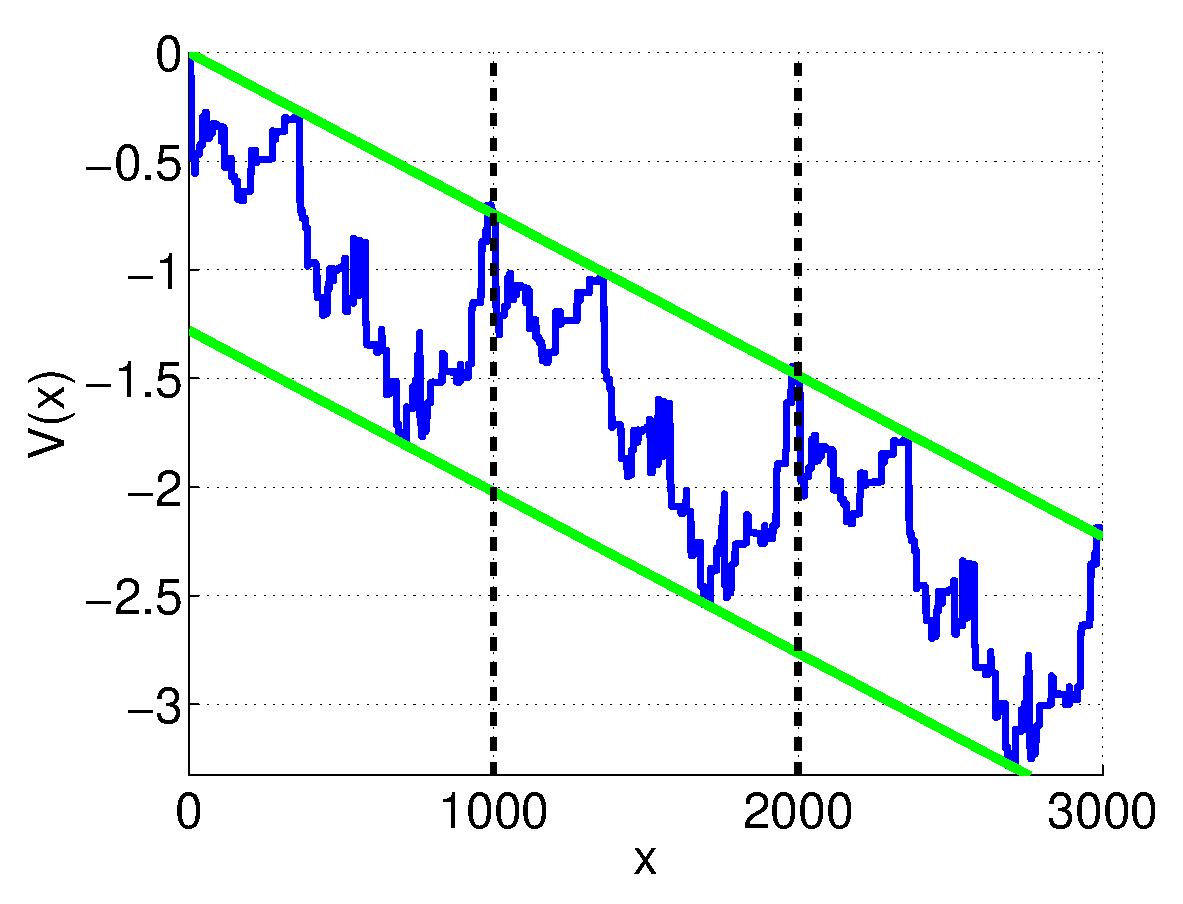
\includegraphics[height=3.5cm]{V_x}

\Dn[2]

[1] {\bf Sinai} (1982)

[2] {\bf Derrida} (1983)

[3] {\bf Aslangul, Pottier, Saint-James}  (1989)

\Dn[2]

\cred{\bf ESR is violated for large $s$}

\emp


\esl


%%%%%%%%%%%%%%%%%%%%%%%%%%%%%%%%%%%%%%%%%%%%%%%%%

\bslC

\Tl{\large{Observations  for finite $N$} }

\bmp{0.5\hsize}

\center{General $N$ }

\includegraphics[height=.7\hsize]{v_D_rat}

\smp{0.5\hsize}

\center{Effective lattice constant ($N=6$)}

\includegraphics[height=.7\hsize]{a_inf}


\emp

\be
\hspace{1cm} \text{\cgreen{Generalized ESR for a given disorder $\sigma$}} \hspace{2cm}  \frac{v}{D} \ = \ \frac{2}{a_s} \tanh \frac{a_s s}{2}
\ee

{\bf \ (1)}~For small values of $s$ we have ${v/D=s}$, in consistency with the ESR. 

%
{\bf \ (2)}~For no disorder ($\sigma=0$) we have ${a_s=1}$, reflecting the discreteness of the lattice. 
%

{\bf \ (3)}~For finite disorder and moderate $s$ we have ${a_s \sim N}$, reflecting the length of the unit cell.
%

{\bf \ (4)}~For finite disorder and large $s$ we have ${a_s=a_{\infty}}$, reflecting the disorder $\sigma$. 
%

{\bf \ (5)}~As $N$ becomes larger our results approach those of [2,3], which we call "Sinai step".



\esl

%%%%%%%%%%%%%%%%%%%%%%%%%%%%%%%%%%%%%%%%%%%%%%%%%
\bslD

\Tl{Outline}


\bmp{0.4\hsize}

\cgreen{General $s$ dependence} 

\smp{0.35\hsize}

\Up\Up
\[  \frac{v}{D} \ = \ \frac{2}{a_{s}}\tanh\frac{a_s s}{2} \]

\smp{0.2\hsize}

\cred{\ \ \ \ $a_{s}: \ N...a_{\infty}$}

\emp

\bmp{0.4\hsize}

\cgreen{Poisson $(s\to \infty)$}

\smp{0.35\hsize}

\Up\Up
\[ \frac{v}{D} \ = \ \frac{2}{a_{\infty}} \]

\smp{0.2\hsize}

\cred{$a_{\infty}(\sigma): \ 1...N$}

\emp



\bmp{0.4\hsize}

\cgreen{ESR $(s\to 0)$}  

\smp{0.35\hsize}

\Up\Up
\[ \frac{v}{D} \ = \ s \]

\smp{0.2\hsize}

\

\emp



\Dn\Dn

{\Huge
\cgreen{\ \ \ Given $\left(1, \ N, \ \sigma \right)$} \ \ \ \ \ \ \ \cred{$a_s \ = \ ? $}
}

\Dn

\Cn{\cgreen{$\sigma$ is the log-width of the stochastic field distribution}}

\esl

%%%%%%%%%%%%%%%%%%%%%%%%%%%%%%%%%%%%%%%%%%%%%%%%%
\bslD

\Tl{\large{Nonequilibrium Fluctuation Theorem (NFT) derivation of the ESR}}

\Dn

\cgreen{Define $x$ as the \cred{winding number} times the length of the ring.}  
%
\[
\frac{P\left[\bm{r}(-t)\right]}{P\left[\bm{r}(t)\right]} \ = \ \exp \left[ -\mathcal{S}[\bm{r}] \right] 
\hspace*{2cm}
\cred{\leadsto}
\hspace*{2cm}
\frac{p(-x;t)}{p(x;t)} \ = \ \eexp{- s x}
\]

\cgreen{Gaussian approximation ({\bf Central Limit Theorem})}
%
\[
p(x;t) \ \approx \ \overline{p}(x;t) \ = \ 
\frac{1}{\sqrt{4\pi Dt}} 
\exp
\left[ 
-\frac{\left(x - v t \right)^2}{4Dt}
\right]
\hspace*{1cm}
\cred{\leadsto}
\hspace*{1cm}
\frac{v}{D} \ = \ s 
\]

\Dn

\center{\cred{\bf Does the ESR really hold?}}
%
%\bmp{0.5\hsize}
%
%{\bf BUT!} in the literature we find
%
%[1-2] (discrete lattice, $N = \infty$) 
%
%[3-4] (continuous washboard potential) 
%%
%\be
%v &=& ...\\
%D &=& ...\\
%\frac{v}{D} &= & f(s) \ \neq \ s
%\ee
%
%\smp{0.5\hsize}
%
%\Dn
%
%\tiny{
%
%[1] Ya. G. Sinai, Theory Probab. Appl. 27, 247 (1982)
%
%[2] B. Derrida, J. Stat. Phys. 31, 3, (1983).
%
%[3] C. Aslangul, N. Pottier and D. Saint-James, J. Phys. France 50, 899-921 (1989).
%
%[4] C. Cattuto and F. Marchesoni, Phys. Rev. Lett. 79, 5070 (1997).
%
%[5] P. Reimann, C. Van den Broeck, H. Linke, P. Hanggi, J. M. Rubi, and A. Perez-Madrid, Phys. Rev. Lett. 87, 010602 (2001).
%}
%\emp
%
%\Dn
%
%\Dn
%
%\begin{itemize}
%\item {\bf Resolution of the "paradox".}
%\item {\bf Physical meaning behind $v, \ D$.}
%\end{itemize}

\esl

%%%%%%%%%%%%%%%%%%%%%%%%%%%%%%%%%%%%%%%%%%%%%%%%
\bslC

\Tl{\large{NFT and coarse graining}}

%\bmp{0.5\hsize}

%All bonds are identical, 
%
%transition rates from left to right are $\ora{w}$,  
%
%transition rates from right to left are $\ola{w}$. 
%
%Total entropy production is $\mathcal{S}_{\circlearrowleft} = \ln(\ora{w}/\ola{w})$

%\smp{0.5\hsize}

\cgreen{Asymmetric random walk traversing a distance  ${x=X_1+...+X_{\mathcal{N}}}$}

\Up

%
\beq
P(X =+1) \ &=& \ p \ \ \equiv \ \ \ora{w}\tau \\
P(X =-1) \ &=& \ q \ \ \equiv \ \ \ola{w}\tau \\
P(X = 0) \ &=& \ 1-p-q 
\eeq

%\emp

\Up

%
\be
\text{\cgreen{Moment generating function }} \ \ \ \ \ \ \ \ \ \ \ \ \ 
\ \ \ Z(k) \  &=&  \ \langle \eexp{-ik x} \rangle \  = \  \left[p\eexp{-ik} + q\eexp{+ik} + (1-p-q)\right]^{\mathcal{N}}\\
\text{\cgreen{In the continuous time limit}} \  p,q\ll 1, 
\ \ \ \ln Z(k)  &= & \mathcal{N} \left[p \eexp{-ik} + q\eexp{+ik} -(p+q) \right]
\ + \  \mathcal{O}(\mathcal{N}\tau^2)
\ee
%

\cgreen{Accordingly, one obtains:}
%
\[
p(x;t) \ \ = \ \ \int_{-\infty}^{\infty}  \!\! dk \ 
\eexp{ ikx + \left(\ora{w} \eexp{-ik} + \ola{w} \eexp{ik} -(\ola{w}+\ora{w})\right)t} \hspace{1cm} \text{\cblue{ satisfies NFT}}
\]

\cgreen{Correct application of the CLT}:
%
\[
\overline{p}(x;t) \ \ = \ \ \int_{-\infty}^{\infty} \!\! dk \
\eexp{ ik (x - (\ora{w}-\ola{w})t) - \frac{k^2}{2}(\ora{w}+\ola{w})t  + \ \ \cred{\text{\sout{$\mathcal{O}(k^3 t)$}}} } \ \ = \ \
\frac{1}{\sqrt{4\pi Dt}} 
\exp
\left[ 
-\frac{\left(x - v t \right)^2}{4Dt}
\right]
\]


\[v \ = \ \ora{w}-\ola{w} \ , \ \ D \ = \ \frac{1}{2}(\ora{w}+\ola{w})
\hspace*{1cm}
\cred{\leadsto}
\hspace*{1cm}
\frac{v}{D} \ = \ \overline{s} \ = \ \frac{2}{a} \tanh \frac{as}{2} \ \ \ \text{\cred{The affinity is renormalized!}}
\]

\cgreen{The naive reasoning, based on CLT, is \cred{wrong}, If we smear $p(x)$ we get} 
%
\[\hspace{5cm}
\frac{\overline{p}(-x;t)}{\overline{p}(x;t)} \ = \ \eexp{- \overline{s} x}
\]

\esl



%%%%%%%%%%%%%%%%%%%%%%%%%%%%%%%%%%%%
\bslC

\Tl{\large{Recipe for computing $v$ and $D$ on a periodic array}}

\cgreen{ Dynamics determined by rate equation: ${(d/dt) \bm{p} = W\bm{p}}$}

{\bf$W$ is not symmetric yet periodic, thus Bloch's theorem applies.}

Reduced equation for the eigenmodes  $\bm{W}(\varphi)\psi = -\lambda\psi$, 
where $\bm{W}(\varphi)$ is an $N\times N$ matrix. 

Bloch's theorem:  $\psi_{n+N}=\eexp{i\varphi}\psi_n$,  where $n$ is the site index mod($N$). 

Bloch quasi-momentum  ${\varphi\equiv kN}$.

Diagonalizing  $\bm{W}(\varphi) \ \ \leadsto \ \{|k,\nu\rangle, -\lambda_{\nu}(k)\}$,
where $\nu$ is the band index.

\Dn

\cgreen{Time dependent solution of the rate equation}

\Up

\be
p_n(t) \ & \approx & \ \frac{1}{L}\sum_{k,\nu} C_{k,\nu} \ \eexp{-\lambda_{\nu}(k) t} \ \eexp{ikn}
\ \ \ \ \text{where} \ \ C_{k,\nu}  \ \ \text{depend on initial conditions.}
\ee

\Dn

\cgreen{In the long time limit only $\lambda_0$ survives}

\Up

\be
v \ &=& \ \left. i \frac{\partial \lambda_0(k)}{\partial k}\right|_{k=0}
\\ 
D \ &=& \ \left. \frac{1}{2} \frac{\partial^2 \lambda_0(k)}{\partial k^2}\right|_{k=0}
\eeq


\esl


%%%%%%%%%%%%%%%%%%%%%%%%%%%%%%%%%%%%%%%%%%%%%%%%%
\hide{
\bslC


\Tl{\large{Minimally disordered ring, $N=2$ sites per unit cell}}

\bmp{0.5\hsize}


The transition rates ${(\ora{A},\ola{A},\ora{B},\ola{B})}$,

 $\ln(\ora{A}/\ola{A})=s{+}\sigma$ 
and ${\ln(\ora{B}/\ola{B})=s{-}\sigma}$

\beq
v \ = \ \frac{\ora{A} \ora{B} - \ola{A} \ola{B}}{ \ora{A} + \ola{A} + \ora{B}+  \ola{B}} 
\eeq
%

\Dn

and

%
\beq
D \ = \ \frac{1}{2}\left[
\frac{\ora{A} \ora{B} + \ola{A} \ola{B}  - 2v^2 }
{ \ora{A}+ \ola{A} + \ora{B}+  \ola{B}}\right] 
\eeq
%

\Dn

The $v/D$ ratio is given by 
%

\beq
\frac{v}{D} \ = \ \frac{2}{1 +  \tanh^2\left(\frac{\sigma}{2}\right)\tanh^2\left(\frac{s}{2}\right)} \tanh\left(\frac{s}{2}\right)
\eeq

\smp{0.5\hsize}

\includegraphics[height=.7\hsize]{v_D_sim.eps}

\cred{As the ``disorder" $\sigma$ increases $\tanh^2({\sigma/2})$ 
grows from~0 to~1, and consequently ${a_{\infty}}$ grows from the 
value ${a=1}$ to the value ${a=2}$. }
\emp

\esl
}

%%%%%%%%%%%%%%%%%%%%%%%%%%%%%%%%%%%%%%%%%%%%%%%%%%%%%%%%%%%


%%%%%%%%%%%%%%%%%%%%%%%%%%%%%%%%%%%%%%%%%%%%%%%%%

%%%%%%%%%%%%%%%%%%%%%%%%%%%%%%%%%%%%%%%%%%%%%%%%%%%%%%%%%%%%%%%%%%%%%%%%%%%%%%%%%%

\bslC

\Tl{\Large{The Poisson Limit $(s\to\infty)$}}



\bmp{0.6\hsize}

\cgreen{The limit $s\to\infty$ corresponds to 
a uni-directional 
\\
random walk traversing a distance } ${x=X_1+...+X_{\mathcal{N}}}$

\Up[3]

\beq
P(X_n = 1) &=& w_n \tau \\
P(X_n = 0) &=& 1-w_n \tau \\
P(X_n=-1) &=&0 
\eeq

\Dn[3]

\cgreen{Characteristic polynomial for eigenvalues of} $\bm{W}(\varphi)$

\Up

\[
\det(\lambda+\bm{W}(\varphi)) 
\ = \ \prod_{n=1}^N (\lambda {-} w_n) + \eexp{-i\varphi} \prod_{n=1}^N w_n 
\ = \ 0 
\]

\smp{0.4\hsize}




\includegraphics[height=.7\hsize]{a_inf.eps}

\center{Effective lattice constant ($N=6$)}


\emp

\Dn[3]

\cgreen{Expanding to second order in} $\lambda$ \cgreen{and } $\varphi$


\Up[3]

\beq
\lambda &=& 
-i \left[\left(\sum_{n=1}^N \frac{1}{w_n} \right)^{-1}\right] \varphi 
\ + \  \frac{1}{2} \left[\left( \sum_{n=1}^N \frac{1}{w_n} \right)^{-3} \left(\sum_{n=1}^N \frac{1}{w_n ^2}\right)\right] \varphi^2 
\ + \ \mathcal{O}(\varphi^3)  
\ee

\Dn

\cgreen{From the recipe for} $v$ \cgreen{and} $D$:

\Up

\[
\cred{a_{\infty} \ \ = \ \  \left(\frac{2D}{v}\right)_{s\rightarrow\infty} \ = \ 
\left[\frac{\big\langle (1/\ora{w})^2 \big\rangle}{\big\langle (1/\ora{w}) \big\rangle^2}\right]}
\ \ = \ \
\text{[For log-box distribution]} \ \ = \  \ \frac{\sigma}{2} \coth\left( \frac{\sigma}{2} \right)
\]



\esl

%%%%%%%%%%%%%%%%%%%%%%%%%%%%%%%%%%%%%%%%%%%%%%%%%
\bslC

\Tl{\large{Spreading analysis and the "Sinai step"} }




\Up

\[
\left\langle  \left(\frac{\overleftarrow{w}}{\overrightarrow{w}}\right)^{\mu}\right\rangle \ \ \equiv \ \ \eexp{-(s-s_{\mu})\mu} \hspace{4cm} [ \ \text{\cgreen{defines}} \ \ s_{\mu} \ ]
\]

{The values $s_{1/2},  \ s_1$ and  $s_2$ determine crossover points between transport regimes.}

\Dn

\cgreen{\bf For $s=0$, anomalous time dependent  spreading} [Sinai],
%

\Up

\[
{x} \ \ \sim \ \ [\log(t)]^2  \hspace{2cm} \cred{\leadsto} \hspace{2cm} v \ \ \sim \ \ e^{-\sqrt{N}}
\]

\Dn

%
\cgreen{\bf For  finite $s<s_1$}  [Bouchaud, Comtet, Georges,  Le Doussal, 1987],
%

\Up


\[
{x} \ \ \sim \ \ t^{\mu} \hspace{5cm} [ \  \cgreen{\mu \text{ is the value for which} \ s_{\mu}=s} \ ]
\]

Time required to drift $x \sim N$ 
is $t \sim N^{1/\mu}$, hence we deduce

\Up

\beq
v \ \ \sim \ \ \frac{x}{t} \ \ \sim \ \ \left(\frac{1}{N}\right)^{\frac{1}{\mu}-1} \ \ 
\eeq

Crossover at $s=s_{1/2}$ from sub-Ohmic to super-Ohmic behaviour.

\Dn

\cgreen{\bf For large  $s>s_1$ and $N\to \infty$} [Derrida],

\Up

\[
v_s \ \ = \ \  
\frac{ 1 - \left\langle (\ola{w}/\ora{w})\right\rangle}
{\left\langle (1/\ora{w}) \right\rangle}
\ \ = \ \ \left[1-\eexp{-(s-s_1)}\right] v_{\infty}  
\]

\esl
%%%%%%%%%%%%%%%%%%%%%%%%%%%%%%%%%%%%%%%%%%%%%%%%%

\bslC

\Tl{\large{The affinity dependent length scale $a_s$ } }

\bmp{0.6\hsize}

\cgreen{From "Derrida" we have an expression for} 
\\
$v$ in the $N\to \infty$ limit.

\Dn 

\cgreen{From our reasoning we have in general }

\Up

\[
\frac{v}{D} \ = \ \frac{2}{a_s} \tanh\frac{a_s s}{2} \ \ \cgreen{\text{with some}} \ \  a_s.
\]

 \Dn

\cgreen{By "reverse engineering" we deduce}

\Up

\[ 
\left\{ \begin{array}{cc}
a_s \sim N, & s<s_2 \\
a_s \ \approx \ \frac{a_{\infty}}{1- \left\langle (\ola{w}/\ora{w})^2\right\rangle}
\ = \ \frac{a_{\infty}}{1-\eexp{-2(s-s_{2})}}, & s>s_2
\end{array}
\right.
\]

\smp{0.4\hsize}

\Dn[0.2]

\includegraphics[height=.8\hsize]{vda.eps}


\emp

\Dn

\begin{table*}
\begin{tabular}{|l||c|c|c|c|c|}
\hline
$s$ regime & $[0, 1/N]$  &  $[1/N, s_{1/2}]$  &  $[s_{1/2}, s_{1}]$  & $[s_{1}, s_{2}]$  & $[s_{2},\infty]$ \\
\hline
$\cgreen{a_s}$ & \cgreen{irrelevant }
& \multicolumn{3}{|c|}{$ \cgreen{a_s \sim  N}$} 
& $\cgreen{a_s \approx \left[1-\eexp{-2(s-s_{2})}\right]^{-1} \!\!\! a_{\infty}}$ \\
\hline
$\cred{v_s}$ & \cred{$v = 2D\,s$} 
&  \multicolumn{2}{|c|}{\cred{$\sim \left(\frac{1}{N}\right)^{\frac{1}{\mu}-1}$}} 
&  \multicolumn{2}{|c|}{\cred{$v_s \approx \left[1-\eexp{-(s-s_1)}\right] v_{\infty}$}} \\
\hline
$\cblue{D}$  
& \cblue{$\sim \exp\left(-\sqrt{N}\right)$} 
& \cblue{$\sim \left(\frac{1}{N}\right)^{\frac{1}{\mu}-2}$ }
& \cblue{$\sim \left(N\right)^{2-\frac{1}{\mu}} $}
& \cblue{$\sim N $ }
& \cblue{$D = \frac{1}{2}a_sv_s$} \\
\hline
\end{tabular}

\end{table*}




\esl

%%%%%%%%%%%%%%%%%%%%%%%%%%%%%%%%

\bslD

\Tl{Summary}


\cgreen{\bf To what extent does the ESR hold? } 

As long as $s<1/N$, for a  disordered lattice.

\cgreen{\bf Can it be derived from the NFT? } 

Yes, provided $s$ is replaced by coarse grained $\bar{s}$.

\cgreen{\bf Non-equilibrium version?} 


\Up


\[
\frac{v}{D} \ = \ \frac{2}{\cred{a_s}} \tanh\frac{\cred{a_s} s}{2}
\]


\Up


\[ 
\left\{ \begin{array}{lr}
v \ \sim  \ \left(\frac{1}{N}\right)^{\frac{1}{\mu}-1}, & s<s_1 \\
v \ \approx \ \left[1-\eexp{-(s-s_1)}\right] v_{\infty}, & s>s_1
\end{array}
\right.
\]

\Up

\[ 
\left\{ \begin{array}{lr}
a_s \ \sim \ N, & s<s_2 \\
a_s \ \approx \ \frac{a_{\infty}}{1- \left\langle (\ola{w}/\ora{w})^2\right\rangle}
\ = \ \frac{a_{\infty}}{1-\eexp{-2(s-s_{2})}}, & s>s_2
\end{array}
\right.
\]






\esl


%%%%%%%%%%%%%%%%%%%%%%%%%%%%%
\hide{
\bslC

\Tl{\Large{Summary and Discussion}}

\Dn


	\begin{enumerate}
	
	\item In general nonequilibirum circumstances, ESR is not valid.
	
	\item For 1D lattice, generalized ESR determined by affinity dependent length-scale $a_s$. 
			$\displaystyle \frac{v}{D} \ =  \ \frac{2}{a_s} \tanh \frac{a_s s}{2}$ 

	
	\item As $s$ increases, $a_s$ drops from the period $N$  to the disorder limited value $a_{\infty}$.
	
	\item Requirement for ESR is $a_s s < 1$, becomes more demanding for large $s$.
	
	\item Apparent NFT - ESR paradox resolved: 
	
	Implicit coarse graining procedure results in effective affinity  $\bar{s}=\ \frac{2}{a} \tanh \frac{a s}{2}$. Replacing $s$ by $\bar{s}$, the generalised ESR is obtained.
	
	\item Experimental relevance of coarse graining in the case of limited resolution of measurement apparatus. Example: Experimental test of NFT for electron transport through a quantum dot.  
	[Nakamura, Yamauchi, Hashisaka, Chida,  Kobayashi, Ono, Leturcq, Ensslin, Saito, Utsumi, Gossard, 2010]
	
	
	\item Apparent violation of NFT explained on basis of existence of secondary circuits [Rahav \& Jarzynski, 2007. Cuetara, Esposito, Schaller, Gaspard, 2011].
	In our model, there are no secondary loops, yet  the bare affinity is replaced by effective affinity.
	
	\end{enumerate}

\esl


}

\bslC

\Tl{Epilog: Experiments}

\begin{itemize}


\item S.H. Lee and D. G. Grier, {\bf Giant Colloidal Diffusivity on Corrugated Optical Vortices}, PRL 2006 

\item Giorgio Volpe, Giovanni Volpe, Sylvain Gigan,
 {\bf Brownian Motion in a Speckle Light Field:
Tunable Anomalous Diffusion and
Selective Optical Manipulation}, Scientific Reports 2014

\item  S. Nakamura, Y. Yamauchi, M. Hashisaka, K. Chida, K.
Kobayashi, T. Ono, R. Leturcq, K. Ensslin, K. Saito, Y. Utsumi, A.C. Gossard, 
{\bf Nonequilibrium fluctuation relations in a quantum coherent conductor
}, PRL 2010

\item B. Kung, C. Rossler, M. Beck, M. Marthaler, D. S. Golubev, Y. Utsumi, T. Ihn, and K. Ensslin {\bf Irreversibility on the Level of Single-Electron Tunneling}, 
PRX 2012

\end{itemize}


\esl

\end{document}




